% !TEX program = xelatex
\documentclass[aspectratio=169,10pt]{beamer}
% !TEX root = main.tex
\usepackage{fontspec}
\setsansfont{TeX Gyre Heros}
\usepackage[spanish,es-nodecimaldot]{babel}
\usepackage{amsmath,booktabs,tabularx,array,graphicx,tikz}
\usetikzlibrary{arrows.meta,positioning,calc,fit,backgrounds,babel}
\definecolor{navy}{HTML}{00547A}
\definecolor{green}{HTML}{6BBB90}
\definecolor{ink}{HTML}{183747}
\definecolor{muted}{HTML}{62747E}
\definecolor{warn}{HTML}{B75940}
\definecolor{violet}{HTML}{756494}
\colorlet{pale}{navy!6!white}
\colorlet{mint}{green!17!white}
\colorlet{warm}{warn!9!white}
\setbeamercolor{normal text}{fg=ink,bg=white}
\setbeamercolor{structure}{fg=navy}
\setbeamercolor{frametitle}{fg=navy}
\setbeamercolor{block body}{fg=ink,bg=pale}
\setbeamerfont{frametitle}{size=\Large,series=\bfseries}
\setbeamertemplate{navigation symbols}{}
\setbeamertemplate{itemize items}{\small\textbullet}
\setbeamersize{text margin left=8mm,text margin right=8mm}
\newcommand{\irycislogo}[1]{
\includegraphics[width=#1,trim={20bp 36bp 21bp 49bp},clip]{assets/logo-irycis-oficial.png}}
\newcommand{\deckpart}{1/6 · Consulta y nota}
\newcommand{\setpart}[1]{\renewcommand{\deckpart}{#1}}
\newif\ifinappendix
\inappendixfalse
\setbeamertemplate{frametitle}{\vspace{2mm}\strut\insertframetitle\strut\par\vspace{1mm}}
\setbeamertemplate{footline}{%
  \hspace{8mm}\textcolor{green}{\rule{.65mm}{2mm}}\hspace{1.5mm}%
  {\color{muted}\fontsize{7}{8}\selectfont\deckpart}%
  \hfill\raisebox{-1mm}[0pt][0pt]{\irycislogo{18mm}}\hfill%
  {\color{muted}\fontsize{7}{8}\selectfont Borrador · 12/10/2026 · \ifinappendix Anexo\else\insertframenumber/31\fi}%
  \hspace{8mm}\vspace{3mm}}
\newcommand{\topic}[1]{{\small\color{muted}#1}\par\vspace{2mm}}
\newcommand{\sources}[1]{\vfill\vspace{1mm}{\fontsize{6.5}{7.7}\selectfont\color{muted}Fuentes: #1\par}}
\newcommand{\link}[2]{\href{#1}{\textcolor{navy}{#2}}}
\newcommand{\takeaway}[1]{\par\vspace{2mm}\begin{beamercolorbox}[sep=1.6mm,wd=\textwidth]{block body}\small #1\end{beamercolorbox}}
\newcommand{\smallnote}[1]{{\fontsize{8}{10}\selectfont\color{muted}#1\par}}
\newcolumntype{L}[1]{>{\raggedright\arraybackslash}p{#1}}
\renewcommand{\tabularxcolumn}[1]{>{\raggedright\arraybackslash}p{#1}}
\renewcommand{\arraystretch}{1.25}
\tikzset{>=Stealth,
  every node/.style={font=\small,text=ink,execute at begin node={\hyphenpenalty=10000\relax\exhyphenpenalty=10000\relax}},
  box/.style={draw=navy!25,fill=pale,rounded corners=2pt,align=center,inner sep=6pt},
  good/.style={box,draw=green!80!navy,fill=mint},
  alert/.style={box,draw=warn!55,fill=warm},
  plain/.style={align=left,inner sep=0pt},
  arr/.style={->,line width=.85pt,draw=navy!80},
  ctx/.style={->,dashed,line width=.85pt,draw=violet},
  tinylabel/.style={font=\scriptsize,text=muted,align=center},
  number/.style={circle,fill=navy,text=white,font=\bfseries\small,minimum size=6mm,inner sep=0pt}}
% Fixed-size figure canvas prevents diagrams from changing slide geometry.
\newenvironment{figurecanvas}[1][4.4]{\begin{center}\begin{tikzpicture}[x=1cm,y=1cm]\path[use as bounding box] (0,0) rectangle (14,#1);}{\end{tikzpicture}\end{center}}
\hypersetup{pdftitle={Construir un escriba digital médico — borrador técnico de 30 minutos},pdfauthor={IRYCIS · Documento de trabajo},colorlinks=true,linkcolor=navy,urlcolor=navy}

\begin{document}

\setpart{1/6 · Consulta y nota}

% 01 — 30s · acumulado 00:30
\begin{frame}[t]
  \vspace{4mm}
  \irycislogo{36mm}\par\vspace{5mm}
  \begin{columns}[T,onlytextwidth]
    \begin{column}{.52\textwidth}
      {\color{navy}\fontsize{27}{30}\selectfont\bfseries Construir un escriba\\digital médico\par}
      \vspace{4mm}
      {\large De la consulta a una nota clínica\par}
      \vspace{5mm}
      \smallnote{Borrador técnico · 30 minutos\\Tareas, evaluación, modelos y ejecución local}
    \end{column}
    \begin{column}{.45\textwidth}
      \begin{tikzpicture}[x=1cm,y=1cm]
        \node[box,text width=1.65cm] (a) at (1,3.2) {Audio};
        \node[box,text width=1.65cm] (c) at (4,3.2) {Contexto clínico};
        \node[good,text width=2.5cm] (n) at (2.5,1.8) {Borrador de nota};
        \node[box,text width=2.5cm] (r) at (2.5,.4) {Revisión clínica};
        \draw[arr] (a)--(n); \draw[ctx] (c)--(n); \draw[arr] (n)--(r);
      \end{tikzpicture}
    \end{column}
  \end{columns}
\end{frame}

% 02 — 45s · acumulado 01:15
\begin{frame}{Objetivo y alcance}

  \topic{Documentar el encuentro y facilitar la revisión del profesional.}
  \begin{figurecanvas}[3.6]
    \node[box,text width=2.2cm] (a) at (1.4,2.8) {Consulta};
    \node[box,text width=2.2cm] (b) at (5,2.8) {Borrador};
    \node[box,text width=2.2cm] (c) at (8.6,2.8) {Revisión};
    \node[good,text width=2.2cm] (d) at (12.2,2.8) {Nota cerrada};
    \draw[arr] (a)--(b); \draw[arr] (b)--(c); \draw[arr] (c)--(d);
    \node[plain,align=center,text width=13cm] at (7,1.65) {\textbf{¿Cómo producir una nota correcta y reducir el trabajo de cerrarla?}};
    \foreach \x/\n/\txt in {1.15/1/{Consulta\\y nota},3.48/2/{Evaluación\\y datos},5.81/3/{Audio y\\hablantes},8.14/4/{Diálogo, contexto\\y nota},10.47/5/{Adaptación\\y despliegue},12.8/6/{Plan de\\trabajo}} {
      \node[number] at (\x,.9) {\n};
      \node[tinylabel] at (\x,.25) {\txt};
    }
  \end{figurecanvas}
  \smallnote{Los escribas humanos documentan bajo supervisión clínica. Algunos productos amplían esta función a informes, codificación o ayuda a decisiones; aquí estudiamos la nota.}
  \sources{\link{https://doi.org/10.1093/jamia/ocaa199}{Ash et al., Safe use of the EHR}; \link{https://pmc.ncbi.nlm.nih.gov/articles/PMC6694617/}{Coiera et al., Taking note}; \link{https://tandemhealth.ai/product/ai-scribe}{Tandem: funciones declaradas del producto}.}

\end{frame}

% 03 — 60s · acumulado 02:15
\begin{frame}{Información del encuentro}
  \topic{Ejemplo ficticio que seguiremos hasta la nota.}
  \begin{figurecanvas}[4.1]
    \node[box,text width=3.7cm,font=\fontsize{9}{11}\selectfont,minimum height=2.4cm] (a) at (2.1,2.65) {\textbf{Conversación}\\[2mm]«Tos desde hace tres días.\\No he tenido fiebre».\\[2mm]Clínico: «Está en mejoría;\\revisión en siete días».};
    \node[box,text width=3.7cm,font=\fontsize{9}{11}\selectfont,minimum height=2.4cm] (b) at (7,2.65) {\textbf{Contexto clínico}\\[2mm]HCIS · antecedentes\\medicación · resultados\\[2mm]«Alergia a penicilina»\\registrada en 2019};
    \node[box,text width=3.7cm,font=\fontsize{9}{11}\selectfont,minimum height=2.4cm] (c) at (11.9,2.65) {\textbf{Observaciones}\\[2mm]Exploración, medidas\\o entrada manual\\[2mm]Temperatura medida hoy:\\36,7 °C};
    \node[good,text width=5.6cm] (d) at (7,.6) {Entradas para generar la nota};
    \draw[arr] (a.south)--(d.west); \draw[ctx] (b.south)--(d.north); \draw[arr] (c.south)--(d.east);
    \node[tinylabel,anchor=west] at (7.2,1.35) {cuando está disponible};
  \end{figurecanvas}
  \takeaway{Conservar quién aporta cada dato, cuándo y de qué fuente procede.}
  \sources{\link{https://pmc.ncbi.nlm.nih.gov/articles/PMC8075472/}{The anatomy of clinical documentation (2021)}; \link{https://arxiv.org/abs/2308.14089}{MedAlign (2023)}. Ejemplo propio.}
\end{frame}

% 04 — 75s · acumulado 03:30
\begin{frame}{La nota SOAP}
  \topic{Una forma habitual de estructurar la nota; las plantillas cambian entre servicios.}
  \begin{figurecanvas}[4.25]
    \foreach \rowY/\rowLetter/\rowName/\rowContent/\rowOrigin in {
      3.65/S/Subjetivo/{Tos de tres días; niega fiebre.}/{Relato del paciente},
      2.68/O/Objetivo/{Temperatura: 36,7 °C.}/{Medición de hoy},
      1.71/A/Valoración/{En mejoría, según valoración clínica.}/{Juicio expresado por el clínico},
      .74/P/Plan/{Revisión en siete días, indicada por el clínico.}/{Decisión expresada en consulta}} {
      \node[number] at (.35,\rowY) {\rowLetter};
      \node[plain,text width=1.8cm] at (1.8,\rowY) {\textbf{\rowName}};
      \node[box,anchor=west,text width=6.7cm,minimum height=.65cm] at (3,\rowY) {\rowContent};
      \node[tinylabel,anchor=west,text width=2.6cm,align=left] at (10.4,\rowY) {\rowOrigin};
    }
  \end{figurecanvas}
  \smallnote{Contexto adicional: alergia registrada en 2019, pendiente de confirmar. Puede aparecer en una sección específica de antecedentes/alergias.}
  \sources{\link{https://www.ncbi.nlm.nih.gov/books/NBK482263/}{SOAP Notes, StatPearls}; \link{https://pmc.ncbi.nlm.nih.gov/articles/PMC8075472/}{The anatomy of clinical documentation}. Ejemplo ficticio; A y P documentan al clínico.}
\end{frame}

% 05 — 50s · acumulado 04:20
\begin{frame}{Pipeline del escriba}

  \topic{Entradas y salidas que podamos inspeccionar.}
  \begin{figurecanvas}[4.05]
    \node[box,text width=1.05cm] (a) at (.75,2.1) {Audio};
    \node[box,text width=1.75cm] (b) at (3.3,2.1) {ASR +\\hablantes};
    \node[good,text width=2.1cm] (c) at (6.6,2.1) {Selección +\\generación};
    \node[box,text width=1.75cm] (d) at (9.8,2.1) {Comprobar\\borrador};
    \node[box,text width=1.45cm] (e) at (12.65,2.1) {Revisión\\clínica};
    \draw[arr] (a)--(b); \draw[arr] (b)--(c); \draw[arr] (c)--(d); \draw[arr] (d)--(e);
    \node[box,text width=3.5cm] (h) at (6.6,3.65) {Contexto clínico disponible};
    \draw[ctx] (h)--(c);
    \node[box,text width=3.5cm] (m) at (6.6,.5) {Observaciones / entrada manual};
    \draw[arr] (m)--(c);
    \node[good,text width=1.45cm] (f) at (12.65,.5) {HCIS};
    \draw[arr] (e)--(f);
    \node[tinylabel,text width=2.3cm] at (3.3,.95) {Texto, tiempos\\y hablantes};
    \node[tinylabel,text width=2.3cm] at (9.8,.8) {Soporte y conflictos\\para revisión};
  \end{figurecanvas}
  \smallnote{La selección de hechos puede ocurrir dentro del generador o quedar explícita. Comprobar el borrador aporta señales de revisión; su fiabilidad también se evalúa.}
  \sources{Diseño de trabajo, no implementación completa. \link{https://doi.org/10.1038/s41746-025-01622-1}{Evaluación clínica por etapas}; \link{https://aclanthology.org/2023.clinicalnlp-1.18/}{Singh et al.}; \link{https://arxiv.org/abs/2501.16672}{VeriFact}. HCIS: sistema de información clínica.}

\end{frame}

\setpart{2/6 · Evaluación y datos}

% 06 — 60s · acumulado 05:20
\begin{frame}{Evaluación}

  \topic{El éxito se mide en la nota y en el trabajo necesario para cerrarla.}
  \begin{figurecanvas}[4.1]
    \node[box,text width=3.4cm,minimum height=.8cm] at (2,3.3) {\textbf{Audio y hablantes}};
    \node[plain,anchor=west,text width=9.1cm] at (4.4,3.3) {¿Se reconocieron las palabras y quién las dijo?\\WER, errores clínicos y atribución.};
    \node[box,text width=3.4cm,minimum height=.8cm] at (2,1.95) {\textbf{Contenido de la nota}};
    \node[plain,anchor=west,text width=9.1cm] at (4.4,1.95) {¿Qué falta, qué sobra y qué se contradice?\\Hechos, negación, sujeto, fecha y soporte.};
    \node[good,text width=3.4cm,minimum height=.8cm] at (2,.6) {\textbf{Uso clínico}};
    \node[plain,anchor=west,text width=9.1cm] at (4.4,.6) {¿Cuánto esfuerzo exige revisar y corregir?\\Tiempo, ediciones e incidencias del flujo.};
  \end{figurecanvas}
  \takeaway{Necesitamos referencias anotadas para medir errores y revisión clínica para valorar su importancia.}
  \sources{\link{https://aclanthology.org/2022.acl-long.394/}{Moramarco et al., evaluación y post-edición}; \link{https://doi.org/10.1038/s41746-025-01622-1}{Marco clínico de evaluación (2025)}.}

\end{frame}

% 07 — 80s · acumulado 06:40
\begin{frame}{Datos de evaluación}
  \topic{Primero referencias estándar; después datos que se acerquen al uso previsto.}
  \begin{columns}[T,onlytextwidth]
    \begin{column}{.32\textwidth}
      \begin{block}{\small 1 · Referencias generales}
        \small\textbf{LibriSpeech}\par 960 h de entrenamiento ASR; inglés leído.\par\vspace{3mm}
        \textbf{AMI}\par Unas 100 h de reuniones; audio y hablantes.\par\vspace{3mm}
        \textbf{FLEURS}\par 102 idiomas, unas 12 h/idioma; incluye español.
      \end{block}
    \end{column}
    \begin{column}{.32\textwidth}
      \begin{block}{\small 2 · Consulta clínica en inglés}
        \small\textbf{PriMock57}\par 57 consultas simuladas; 8 h 38 min; audio, turnos y notas.\par\vspace{3mm}
        \textbf{ACI-Bench}\par 207 encuentros simulados; transcripciones y notas; sin audio público.\par\vspace{3mm}
        \textbf{MTS-Dialog}\par 1.701 pares breves diálogo–sección.
      \end{block}
    \end{column}
    \begin{column}{.32\textwidth}
      \begin{block}{\small 3 · Aproximación al español clínico}
        \small\textbf{TEME-v1}\par 90 diálogos, 2.330 turnos, 3,96 h de audio TTS; dos voces.\par\vspace{3mm}
        Útil para explorar ASR; sin tiempos de referencia para evaluar DER directamente.\par\vspace{3mm}
        \textbf{Conjunto local propuesto}\par Consultas y notas revisadas del escenario de uso.
      \end{block}
    \end{column}
  \end{columns}
  \sources{\link{https://www.openslr.org/12}{LibriSpeech}; \link{https://groups.inf.ed.ac.uk/ami/corpus/}{AMI}; \link{https://arxiv.org/abs/2205.12446}{FLEURS}; \link{https://github.com/babylonhealth/primock57}{PriMock57}; \link{https://github.com/microsoft/clinical_visit_note_summarization_corpus}{ACI}; \link{https://github.com/abachaa/MTS-Dialog}{MTS}; \link{https://zenodo.org/records/17280661}{TEME}. Horas TEME: suma local de los 90 MP3.}
\end{frame}

\setpart{3/6 · Audio y hablantes}

% 08 — 70s · acumulado 07:50
\begin{frame}{Señal y representación acústica}

  \topic{«She just had a baby»: la misma frase en onda y espectrograma.}
  \begin{columns}[T,onlytextwidth]
    \begin{column}{.49\textwidth}
      \small\textbf{Onda y alineamiento}\par\vspace{1mm}
      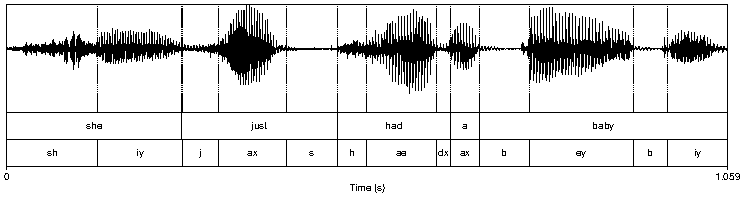
\includegraphics[width=\textwidth,height=3.15cm,keepaspectratio]{figures/jurafsky-wave.pdf}
    \end{column}
    \begin{column}{.49\textwidth}
      \small\textbf{Espectrograma}\par\vspace{1mm}
      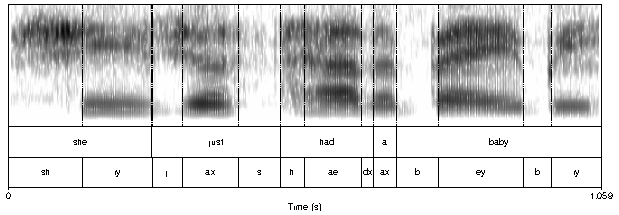
\includegraphics[width=\textwidth,height=3.15cm,keepaspectratio]{figures/jurafsky-spectrogram.pdf}
    \end{column}
  \end{columns}
  \vspace{2mm}
  \begin{columns}[T,onlytextwidth]
    \begin{column}{.32\textwidth}\small\textbf{Captura}\par Canales, muestreo, ruido y compresión.\end{column}
    \begin{column}{.32\textwidth}\small\textbf{Ventanas}\par Analizar cómo cambia el espectro con el tiempo.\end{column}
    \begin{column}{.32\textwidth}\small\textbf{Entrada del modelo}\par Log-Mel, o representación aprendida de la onda.\end{column}
  \end{columns}
  \sources{\link{https://web.stanford.edu/~jurafsky/slp3/15.pdf}{Jurafsky y Martin, cap. 15, figs. 15.15 y 15.22}, borrador 19/08/2026. Recortes del libro; habla de Switchboard en inglés, no consulta clínica. \link{https://arxiv.org/abs/2212.04356}{Whisper}: entrada log-Mel.}

\end{frame}

% 09 — 90s · acumulado 09:20
\begin{frame}{Modelos de ASR}

  \topic{Cómo pasar de estados acústicos a una secuencia de texto.}
  \begin{figurecanvas}[4.3]
    % Own schematic: reference milestones and mechanisms, not a replacement timeline.
% Input inside figurecanvas[4.3].
\begin{scope}[every node/.append style={font=\fontsize{9}{11}\selectfont}]
  \draw[navy!15] (4.6,.25)--(4.6,4.2);
  \draw[navy!15] (9.35,.25)--(9.35,4.2);
  \node[plain,align=center,font=\bfseries\small] at (2.2,3.95) {CTC · 2006};
  \node[plain,align=center,font=\bfseries\small] at (6.95,3.95) {RNN-T · 2012};
  \node[plain,align=center,font=\bfseries\small] at (11.8,3.95) {Atención · 2015};
  \node[box,text width=3.35cm] (a) at (2.2,2.85) {Encoder acústico\\→ etiqueta por frame};
  \node[good,text width=3.35cm] (b) at (2.2,1.65) {Colapsar repeticiones\\y símbolos blank};
  \draw[arr] (a)--(b);
  \node[plain,align=center,text width=4.1cm] at (2.2,.55) {\textbf{Ejemplo}\\Parakeet-CTC};
  \node[box,text width=3.4cm] (c) at (6.95,2.85) {Estado de audio\\+ predictor del texto};
  \node[good,text width=3.4cm] (d) at (6.95,1.65) {Emitir token\\o avanzar en el audio};
  \draw[arr] (c)--(d);
  \node[plain,align=center,text width=4.2cm] at (6.95,.55) {\textbf{Derivado actual}\\Parakeet-TDT v3};
  \node[box,text width=3.45cm] (e) at (11.8,2.85) {Audio codificado\\+ texto anterior};
  \node[good,text width=3.45cm] (f) at (11.8,1.65) {Decoder con atención\\→ siguiente token};
  \draw[arr] (e)--(f);
  \node[plain,align=center,text width=4.2cm] at (11.8,.55) {\textbf{Ejemplos}\\Whisper · Canary};
\end{scope}

  \end{figurecanvas}
  \smallnote{Elegir un modelo concreto exige medir español clínico, velocidad y memoria. La familia de arquitectura por sí sola no determina su calidad.}
  \sources{Esquema propio: \link{https://web.stanford.edu/~jurafsky/slp3/16.pdf}{Jurafsky y Martin, cap. 16}; \link{https://arxiv.org/abs/2303.03329}{Prabhavalkar et al., survey}; \link{https://arxiv.org/abs/2212.04356}{Whisper}. Ejemplo de caracteres simplificado.}

\end{frame}

% 10 — 70s · acumulado 10:30
\begin{frame}{WER y errores clínicos}
  \topic{Referencia: «el paciente no refiere fiebre desde ayer» · 7 palabras.}
  \begin{figurecanvas}[3.75]
    \node[plain,anchor=west] at (.2,3.4) {\textbf{A · Sustitución}};
    \node[box,anchor=west,text width=8.7cm,align=left] at (.2,2.65) {\textcolor{warn}{\textbf{este}} paciente no refiere fiebre desde ayer};
    \node[plain,anchor=west] at (.2,1.7) {\textbf{B · Omisión de una negación}};
    \node[alert,anchor=west,text width=8.7cm,align=left] at (.2,.95) {el paciente \textcolor{warn}{\textbf{[---]}} refiere fiebre desde ayer};
    \node[good,text width=3cm,minimum height=1.8cm] at (12,2) {$\mathrm{WER}=\frac{S+D+I}{N}$\\[4mm]Ambos: $1/7=0{,}143$\\14,3\,\%};
  \end{figurecanvas}
  \smallnote{S: sustituciones · D: eliminaciones · I: inserciones · N: palabras de referencia.}
  \takeaway{Añadir revisión de entidades, negaciones, dosis, fechas y su impacto clínico. El WER sigue siendo útil para diagnosticar ASR.}
  \sources{Definición y cálculo: \link{https://github.com/jitsi/jiwer}{JiWER}; evaluación médica: \link{https://arxiv.org/abs/2406.12387}{Medical ASR benchmark (2024)}; \link{https://doi.org/10.65109/RHNT7438}{TEME}. Ejemplo propio.}
\end{frame}

% 11 — 60s · acumulado 11:30
\begin{frame}{Diarización: tiempo, hablante y rol}
  \topic{Un identificador de hablante no identifica por sí mismo a una persona ni su rol clínico.}
  \begin{figurecanvas}[4.2]
    \node[plain,anchor=west] at (.1,3.8) {\textbf{1. Quién habla y cuándo}};
    \draw[arr] (2,3.05)--(13.5,3.05);
    \foreach \x/\t in {2/0,4.7/2,7.4/4,10.1/6,12.8/8}{\node[tinylabel] at (\x,2.8){\t\ s};}
    \node[tinylabel,anchor=east] at (1.8,2.3) {Hablante S1};
    \node[tinylabel,anchor=east] at (1.8,1.75) {Hablante S2};
    \fill[navy!65,rounded corners=2pt] (2.2,2.12) rectangle (5.9,2.48);
    \fill[navy!65,rounded corners=2pt] (9.5,2.12) rectangle (12.9,2.48);
    \fill[green,rounded corners=2pt] (5.4,1.57) rectangle (10,1.93);
    \draw[warn,dashed] (5.4,1.45) rectangle (5.9,2.6);
    \draw[warn,dashed] (9.5,1.45) rectangle (10,2.6);
    \node[tinylabel,text=warn] at (7.4,1.22) {solapamientos};
    \node[box,text width=5.5cm] at (3.2,.4) {\textbf{2. Qué dice}\\S1: «¿Ha tenido fiebre?»};
    \node[good,text width=5.5cm] at (10.4,.4) {\textbf{3. Qué rol tiene}\\S1: clínico · S2: paciente, tras validarlo};
  \end{figurecanvas}
  \sources{\link{https://arxiv.org/abs/2012.01477}{DIHARD III}; \link{https://github.com/nryant/dscore}{dscore}. Línea temporal ilustrativa; el rol es una etiqueta adicional.}
\end{frame}

% 12 — 80s · acumulado 12:50
\begin{frame}{Modelos de diarización}
  \topic{Dos familias; ruido, turnos cortos y solapamiento ponen a prueba ambas.}
  \begin{figurecanvas}[4.1]
    \node[plain,anchor=west] at (.2,3.9) {\textbf{Modular}};
    \node[box,text width=2.65cm] (a) at (1.7,3) {Voz / segmentación};
    \node[box,text width=2.65cm] (b) at (5.4,3) {Embeddings de voz};
    \node[good,text width=2.65cm] (c) at (9.1,3) {Clustering};
    \node[tinylabel,text width=2cm] (d) at (12.55,3) {S1, S2…\\por intervalo};
    \draw[arr] (a)--(b); \draw[arr] (b)--(c); \draw[arr] (c)--(d);
    \node[plain,anchor=west] at (.2,1.9) {\textbf{End-to-end neural diarization (EEND)}};
    \node[box,text width=2.65cm] (e) at (1.7,.95) {Secuencia acústica};
    \node[box,text width=2.65cm] (f) at (5.4,.95) {Red temporal};
    \node[good,text width=3.6cm] (g) at (10.05,.95) {Actividad por frame y hablante\\S1: 1 1 0 1 · S2: 0 1 1 0};
    \draw[arr] (e)--(f); \draw[arr] (f)--(g);
  \end{figurecanvas}
  \smallnote{\textbf{Modular:} etapas sustituibles; el agrupamiento necesita suficiente evidencia de voz. \textbf{EEND:} modela actividad simultánea; la generalización al número de hablantes y sesiones largas depende del modelo. \textbf{Medir:} DER/JER, con tolerancia temporal y solapamiento definidos.}
  \sources{\link{https://arxiv.org/abs/1909.05952}{Fujita et al., EEND (2019)}; \link{https://www.isca-archive.org/interspeech_2023/plaquet23_interspeech.html}{Plaquet y Bredin, powerset (2023)}; \link{https://huggingface.co/pyannote/speaker-diarization-community-1}{pyannote}; \link{https://arxiv.org/abs/2110.04410}{TitaNet}.}
\end{frame}

% 13 — 50s · acumulado 13:40
\begin{frame}{Transcripción con hablantes}
  \topic{La transcripción diarizada puede ser modular o conjunta.}
  \begin{figurecanvas}[4.05]
    \node[box,text width=1.3cm] (a) at (.9,2.65) {Audio};
    \node[box,text width=3cm] (b) at (4.4,3.45) {ASR + diarización\\+ alineación};
    \node[good,text width=3cm] (c) at (4.4,1.95) {Modelo conjunto\\ej.: MOSS*};
    \node[box,text width=5.7cm,align=left] (d) at (10.8,2.65) {\texttt{[00:02--00:04] [S1]}\\«¿Ha tenido fiebre?»\\[2mm]\texttt{[00:04--00:06] [S2]}\\«No he tenido fiebre».};
    \draw[arr] (a.east)--++(.4,0)|-(b.west); \draw[arr] (a.east)--++(.4,0)|-(c.west);
    \draw[arr] (b.east)--(d.west); \draw[arr] (c.east)--(d.west);
    \node[tinylabel,text width=13cm] at (7,.55) {cpWER: texto con atribución de hablante · tcpWER: añade restricciones temporales\\Comparar reconocimiento, atribución y coste en consultas clínicas.};
  \end{figurecanvas}
  \smallnote{* MOSS-Transcribe-Diarize. Salida ilustrativa; las etiquetas no establecen por sí solas los roles.}
  \sources{\link{https://arxiv.org/abs/2601.01554}{MOSS-Transcribe-Diarize (2026)}; \link{https://github.com/fgnt/meeteval}{MeetEval}. Salida ilustrativa.}
\end{frame}

\setpart{4/6 · Diálogo, contexto y nota}

% 14 — 60s · acumulado 14:40
\begin{frame}{Generación de notas}

  \topic{Primero definir qué documentar y cómo debe verse la salida.}
  \begin{figurecanvas}[4.05]
    \node[box,text width=3.3cm,minimum height=2cm] (a) at (2,2.4) {\textbf{Entradas}\\[3mm]Transcripción y hablantes\\Contexto disponible\\Observaciones};
    \node[good,text width=3.3cm,minimum height=2cm] (b) at (7,2.4) {\textbf{Generador}\\[3mm]LLM + instrucciones\\Plantilla del servicio\\Criterios de contenido};
    \node[box,text width=3.3cm,minimum height=2cm] (c) at (12,2.4) {\textbf{Borrador}\\[3mm]Secciones de la nota\\Hechos y procedencia\\Valoración y plan expresados};
    \draw[arr] (a)--(b); \draw[arr] (b)--(c);
    \node[tinylabel,text width=12cm] at (7,.6) {El equipo clínico define contenido, estilo y errores relevantes; esas decisiones se convierten en instrucciones y criterios de evaluación.};
  \end{figurecanvas}
  \takeaway{Comparar plantillas y prompts sobre los mismos encuentros antes de decidir si hace falta adaptar pesos.}
  \sources{\link{https://www.nature.com/articles/s41597-023-02487-3}{ACI-Bench}; \link{https://aclanthology.org/2022.acl-long.394/}{Moramarco et al.}. Baseline propuesto para el proyecto.}

\end{frame}

% 15 — 100s · acumulado 16:20
\begin{frame}{Selección de hechos}

  \topic{La relevancia puede decidirse al redactar o representarse antes de la nota.}
  \begin{figurecanvas}[4.1]
    \node[box,text width=2cm] (a) at (1.25,2.65) {Diálogo\\+ contexto};
    \node[good,text width=3.2cm] (b) at (6.4,3.4) {Generación directa};
    \node[box,text width=3.2cm] (c) at (6.4,1.8) {Hechos con fuente\\+ diálogo + contexto};
    \node[good,text width=1.7cm] (d) at (12.5,2.65) {Nota};
    \draw[arr] (a.north)|-(b.west); \draw[arr] (b.east)-|(d.north);
    \draw[arr] (a.south)|-(c.west); \draw[arr] (c.east)-|(d.south);
    \node[plain,align=center,text width=13.2cm] at (7,.65) {«Mi madre toma X» $\rightarrow$ \textbf{sujeto: madre}, no paciente\\Hecho · sujeto · negación · momento · fragmento de soporte};
  \end{figurecanvas}
  \smallnote{ASCRIBE: hechos + soporte + relevancia. KOSMOS: entidades, atributos y relaciones. Son estrategias para comparar; la extracción puede introducir omisiones.}
  \sources{\link{https://arxiv.org/abs/2610.01234}{ASCRIBE (2026, preprint; tailandés)}; \link{https://doi.org/10.3390/info17040355}{KOSMOS (2026)}; antecedente: \link{https://aclanthology.org/2023.clinicalnlp-1.18/}{Chain-of-Clinical-Facts, Nuance (2023)}. Sin validación local en español.}

\end{frame}

% 16 — 90s · acumulado 17:50
\begin{frame}{Contexto de la historia clínica}

  \topic{Seleccionar registros externos es una tarea distinta de extraer hechos del diálogo.}
  \begin{figurecanvas}[4.15]
    \node[box,text width=2.4cm,minimum height=1.4cm] (a) at (1.55,2.6) {Historia\\medicación, alergias,\\notas y resultados};
    \node[box,text width=2.4cm,minimum height=1.4cm] (b) at (5.1,2.6) {Identificar paciente\\y encuentro\\fijar corte temporal};
    \node[box,text width=2.4cm,minimum height=1.4cm] (c) at (8.65,2.6) {Seleccionar\\consulta estructurada\\o retrieval};
    \node[good,text width=2.4cm,minimum height=1.4cm] (d) at (12.2,2.6) {Contexto para\\generar la nota\\con fuente y fecha};
    \draw[arr] (a)--(b); \draw[arr] (b)--(c); \draw[ctx] (c)--(d);
    \node[alert,text width=12.2cm] at (7,.75) {2021: «X activa» · 2025: «X suspendida» · hoy: el paciente dice tomar X\\Conservar la discrepancia para revisión; no resolverla por similitud textual.};
  \end{figurecanvas}
  \smallnote{Conservar antecedentes relevantes de otros episodios. Contexto corto: selección estructurada; historia extensa: comparar retrieval. Medir relevancia, vigencia y efecto en la nota.}
  \sources{Diseño propuesto. \link{https://arxiv.org/abs/2005.11401}{RAG}; \link{https://hl7.org/fhir/R4/provenance.html}{FHIR Provenance}. \link{https://arxiv.org/abs/2308.14089}{MedAlign} estudia instrucciones sobre EHR, no valida este conector ni recuperador.}

\end{frame}

% 17 — 90s · acumulado 19:20
\begin{frame}{Comprobaciones de la nota}
  \topic{¿Qué respalda cada afirmación y qué información relevante falta?}
  \begin{figurecanvas}[4.05]
    \node[plain,anchor=west,font=\bfseries] at (.2,3.7) {Afirmación de la nota};
    \node[plain,anchor=west,font=\bfseries] at (7.6,3.7) {Comprobación};
    \node[box,anchor=west,text width=5.5cm,align=left] (a) at (.2,2.9) {«Niega fiebre»};
    \node[good,anchor=west,text width=5.6cm,align=left] (b) at (7.6,2.9) {Soporte: lo refiere el paciente};
    \node[box,anchor=west,text width=5.5cm,align=left] (c) at (.2,1.85) {«Toma actualmente X»};
    \node[alert,anchor=west,text width=5.6cm,align=left] (d) at (7.6,1.85) {Conflicto: figura suspendida en el contexto};
    \node[box,anchor=west,text width=5.5cm,align=left] (e) at (.2,.8) {«Auscultación normal»};
    \node[alert,anchor=west,text width=5.6cm,align=left] (f) at (7.6,.8) {Sin soporte en las entradas disponibles};
    \draw[arr] (a)--(b); \draw[arr] (c)--(d); \draw[arr] (e)--(f);
  \end{figurecanvas}
  \takeaway{Se puede buscar soporte sin nota gold por caso. Medir si el verificador acierta y qué omite exige una muestra anotada.}
  \sources{\link{https://arxiv.org/abs/2501.16672}{VeriFact}; \link{https://github.com/som-shahlab/factehr}{FactEHR}; \link{https://aclanthology.org/2025.emnlp-industry.104/}{Evaluación mediante checklists (2025)}. Ejemplos ficticios.}
\end{frame}

% 18 — 60s · acumulado 20:20
\begin{frame}{Propagación de errores}
  \topic{Propagación ilustrativa: una transcripción errónea puede producir una nota muy fluida.}
  \begin{figurecanvas}[4.1]
    \node[box,text width=2.5cm] (a) at (1.6,2) {Audio\\«No he tenido fiebre»};
    \node[good,text width=3.2cm] (b) at (6.5,3.15) {Transcripción de referencia\\«No he tenido fiebre»};
    \node[alert,text width=3.2cm] (c) at (6.5,.95) {ASR con omisión\\«He tenido fiebre»};
    \node[good,text width=3cm] (d) at (11.85,3.15) {Nota posible\\«Niega fiebre»};
    \node[alert,text width=3cm] (e) at (11.85,.95) {Nota posible\\«Refiere fiebre»};
    \draw[arr] (a.north)|-(b.west); \draw[arr] (a.south)|-(c.west);
    \draw[arr] (b)--node[tinylabel,above]{mismo}(d);
    \draw[arr] (c)--node[tinylabel,above]{generador}(e);
  \end{figurecanvas}
  \takeaway{Si generador y verificador leen el mismo ASR erróneo, pueden compartir el fallo. Conservar el vínculo con el audio.}
  \sources{\link{https://proceedings.mlr.press/v333/latif26a.html}{Latif et al., Robust SOAP (2026)}; \link{https://doi.org/10.1038/s41746-025-01622-1}{Marco de evaluación clínica (2025)}. Esquema causal propuesto; sin resultados experimentales.}
\end{frame}

% 19 — 90s · acumulado 21:50
\begin{frame}{Experimento por etapas}
  \topic{Casos con referencias: mantener generador y plantilla; variar una entrada.}
  \vspace{1mm}
  {\small\renewcommand{\arraystretch}{1.05}
  \begin{tabularx}{\textwidth}{L{.5cm}XXX L{3.2cm}}
    \toprule
    & \textbf{Texto} & \textbf{Hablantes} & \textbf{Contexto} & \textbf{Comparación}\\
    \midrule
    A & Referencia & Referencia & Validado & Entradas revisadas\\
    B & ASR & Referencia & Validado & A→B: sensibilidad a ASR\\
    C & ASR & Predichos & Validado & B→C: sensibilidad a atribución\\
    D & ASR & Predichos & Recuperado & C→D: sensibilidad al contexto\\
    \bottomrule
  \end{tabularx}}
  \vspace{3mm}
  \begin{columns}[T,onlytextwidth]
    \begin{column}{.47\textwidth}\small\textbf{Datos separados}\par Separar ajuste y test por paciente/encuentro; las variantes sintéticas del mismo caso van juntas.\end{column}
    \begin{column}{.49\textwidth}\small\textbf{Evaluación compartida}\par Revisión clínica con rúbrica: errores y edición. Alinear palabras ASR con hablantes de referencia.\end{column}
  \end{columns}
  \sources{Diseño propuesto, inspirado en \link{https://proceedings.mlr.press/v333/latif26a.html}{Robust SOAP}; \link{https://aclanthology.org/2022.acl-long.394/}{Moramarco et al.}; \link{https://doi.org/10.1038/s41746-025-01622-1}{evaluación por etapas}. Requiere referencias alineadas; las diferencias dependen del resto de la configuración.}
\end{frame}

\setpart{5/6 · Adaptación y despliegue}

% 20 — 80s · acumulado 23:10
\begin{frame}{Qué adaptar y con qué datos}

  \topic{La intervención debe responder a un fallo observado.}
  \begin{figurecanvas}[4.1]
    \node[plain,anchor=west,font=\bfseries] at (.2,3.75) {Problema medido};
    \node[plain,anchor=west,font=\bfseries] at (4.7,3.75) {Intervención candidata};
    \node[plain,anchor=west,font=\bfseries] at (9.5,3.75) {Datos y comprobación};
    \foreach \yy/\leftt/\midd/\rightt in {
      2.95/{Terminología médica\\y acento en ASR}/{Configuración, vocabulario\\o fine-tuning ASR}/{Audio + texto revisado\\test clínico español},
      1.8/{Estilo, selección de hechos\\o uso del contexto}/{Plantilla, prompt, extracción\\o adaptación del generador}/{Diálogo/contexto + nota\\criterios de clínicos},
      .65/{Latencia o memoria\\insuficientes}/{Motor, tamaño de modelo\\o cuantización}/{Mismos casos y hardware\\calidad + tiempo + memoria}} {
      \node[box,anchor=west,text width=3.5cm,minimum height=.75cm] (left\yy) at (.2,\yy) {\leftt};
      \node[box,anchor=west,text width=3.7cm,minimum height=.75cm] (mid\yy) at (4.7,\yy) {\midd};
      \node[good,anchor=west,text width=3.55cm,minimum height=.75cm] (right\yy) at (9.5,\yy) {\rightt};
    }
  \end{figurecanvas}
  \sources{Plan propuesto. \link{https://arxiv.org/abs/2212.04356}{Whisper}; \link{https://arxiv.org/abs/2106.09685}{LoRA}; \link{https://arxiv.org/abs/2610.01234}{ASCRIBE: adaptación de generación}; \link{https://github.com/SYSTRAN/faster-whisper}{faster-whisper}. Losses de entrenamiento en anexo B.}

\end{frame}

% 21 — 65s · acumulado 24:15
\begin{frame}{Recursos para ejecución local}

  \topic{Órdenes de magnitud para elegir qué medir; no son un presupuesto del sistema.}
  \begin{figurecanvas}[4.1]
    \node[plain,anchor=west,font=\bfseries] at (.2,3.75) {Whisper: VRAM aproximada};
    \foreach \yy/\name/\gb/\ww in {2.95/small/2/1.05,2.15/medium/5/2.6,1.35/large/10/5.2} {
      \node[plain,anchor=west] at (.2,\yy) {\name};
      \fill[navy!65,rounded corners=2pt] (1.75,\yy-.19) rectangle (1.75+\ww,\yy+.19);
      \node[plain,anchor=west,font=\scriptsize] at (1.95+\ww,\yy) {$\approx$\gb\ GB};
    }
    \node[good,text width=5.1cm,minimum height=1.6cm] at (11.1,2.6) {\textbf{LLM de 7B: solo pesos}\\[3mm]FP16: $\approx$14 GB\\4 bits: $\approx$3,5 GB};
    \node[plain,align=center,text width=5.7cm] at (11.1,1.05) {Añadir KV cache, buffers,\\ASR/diarización y concurrencia.};
    \node[tinylabel,text width=13cm] at (7,.25) {El motor y la precisión cambian consumo y velocidad. Cuantizar exige volver a medir calidad.};
  \end{figurecanvas}
  \sources{\link{https://github.com/openai/whisper}{Whisper README: estimaciones de su implementación}. Cálculo nominal de pesos 7B: parámetros × bits / 8, GB decimales; no medición. \link{https://github.com/ggml-org/whisper.cpp}{whisper.cpp}.}

\end{frame}

% 22 — 65s · acumulado 25:20
\begin{frame}{Scribnic: núcleo y clientes}

  \topic{Base del proyecto actual y ampliaciones propuestas.}
  \begin{figurecanvas}[4.1]
    \node[box,text width=2.35cm] (a) at (1.55,2.6) {CLI actual};
    \node[good,text width=4.35cm,minimum height=2.25cm] (b) at (7,2.6) {\textbf{Core Python existente}\\[3mm]Contratos de audio y spans\\Backends ASR, diarización\\y reconocimiento conjunto\\Generación opcional};
    \node[box,text width=2.55cm] (c) at (12.4,3.25) {Runner de evaluación\\\textcolor{muted}{propuesto}};
    \node[box,text width=2.55cm] (d) at (12.4,1.75) {Cliente desktop\\\textcolor{muted}{propuesto}};
    \draw[arr] (a)--(b); \draw[ctx] (b.east)--(c.west); \draw[ctx] (b.east)--(d.west);
    \node[tinylabel,text width=12.5cm] at (7,.6) {Pendiente: contrato de contexto clínico, referencias/métricas y cliente de revisión.\\Los adaptadores y tests de contratos no demuestran calidad clínica.};
  \end{figurecanvas}
  \sources{Inspección del código local (10/10/2026): \texttt{mypipe/src/scribnic/core.py}, \texttt{models.py}, \texttt{factory.py} y \texttt{README.md}. Estado del proyecto; no resultados de evaluación.}

\end{frame}

% 23 — 75s · acumulado 26:35
\begin{frame}{Captura e integración}

  \topic{La plataforma determina cómo llega la información y cómo se revisa.}
  \begin{figurecanvas}[4.15]
    \node[box,text width=3.3cm,minimum height=1.6cm] (a) at (2,2.8) {\textbf{Captura}\\[3mm]PC, web, móvil\\USB / Bluetooth\\Teleconsulta};
    \node[box,text width=3.3cm,minimum height=1.6cm] (b) at (7,2.8) {\textbf{Procesamiento}\\[3mm]Local, servidor o mixto\\Archivos o streaming\\Colas y recuperación de cortes};
    \node[good,text width=3.3cm,minimum height=1.6cm] (c) at (12,2.8) {\textbf{Revisión y HCIS}\\[3mm]Edición por secciones\\Lectura de contexto\\Escritura de nota aprobada};
    \draw[arr] (a)--(b); \draw[arr] (b)--(c);
    \node[plain,align=center,text width=4.1cm] at (2,.85) {Canales, codec, muestreo\\y pérdidas de audio};
    \node[plain,align=center,text width=4.1cm] at (7,.85) {Qué datos se guardan,\\dónde y por cuánto tiempo};
    \node[plain,align=center,text width=4.1cm] at (12,.85) {Integrar la interfaz no implica\\leer la historia del paciente};
  \end{figurecanvas}
  \sources{\link{https://developer.mozilla.org/en-US/docs/Web/API/MediaDevices/getUserMedia}{Captura web}; \link{https://www.w3.org/TR/webrtc/}{WebRTC}; \link{https://hl7.org/fhir/R4/documentreference.html}{FHIR DocumentReference}; \link{https://tandemhealth.ai/product/ai-scribe}{Tandem: edición por voz y documentos}. Opciones de diseño, no conectores implementados.}

\end{frame}

% 24 — 65s · acumulado 27:40
\begin{frame}{Evaluación del sistema desplegado}

  \topic{Comprobar calidad y funcionamiento en la configuración de uso.}
  \begin{figurecanvas}[4.1]
    \node[box,text width=2.6cm] (a) at (1.65,2.65) {Casos y referencias\\fijados};
    \node[box,text width=3.5cm] (b) at (6.5,3.3) {Entorno experimental\\modelo + prompt + motor};
    \node[box,text width=3.5cm] (c) at (6.5,1.9) {Entorno de despliegue\\hardware + precisión + captura};
    \node[good,text width=3.2cm,minimum height=2.1cm] (d) at (12,2.65) {Errores de la nota\\Latencia p50 / p95\\Tiempo de proceso/audio\\Memoria y concurrencia};
    \draw[arr] (a.east)--++(.35,0)|-(b.west); \draw[arr] (a.east)--++(.35,0)|-(c.west);
    \draw[arr] (b.east)--(d.west); \draw[arr] (c.east)--(d.west);
    \node[tinylabel,text width=12.5cm] at (7,.45) {Después de cada cambio, repetir la evaluación. En piloto: fallos, ediciones y muestra revisada de calidad.};
  \end{figurecanvas}
  \sources{Protocolo propuesto. \link{https://github.com/SYSTRAN/faster-whisper}{faster-whisper}; \link{https://github.com/ggml-org/whisper.cpp}{whisper.cpp}. Sin benchmark de rendimiento local todavía.}

\end{frame}

\setpart{6/6 · Plan de trabajo}

% 25 — 75s · acumulado 28:55
\begin{frame}{Datos del primer experimento}

  \topic{Propuesta acotada para probar el protocolo; no validar todavía el producto.}
  \begin{figurecanvas}[4.2]
    \node[box,text width=3.6cm,minimum height=3.4cm] at (2.1,2.45) {\textbf{1 · Componentes}\\[2mm]TEME: ASR español TTS\\PriMock57: audio, turnos\\y notas en inglés\\[2mm]Referencias públicas};
    \node[box,text width=3.6cm,minimum height=3.4cm] at (7,2.45) {\textbf{2 · Contexto y nota}\\[2mm]10 casos con contexto\\5 consultas PriMock\\adaptadas al español\\[2mm]Referencias revisadas};
    \node[good,text width=3.6cm,minimum height=3.4cm] at (11.9,2.45) {\textbf{3 · Protocolo clínico}\\[2mm]Hechos y fuentes esperados\\Errores, omisiones y edición\\Acuerdo entre revisores\\[2mm]Test separado del ajuste};
    \node[tinylabel,text width=13cm] at (7,.25) {Números propuestos para una prueba de viabilidad. Datos sintéticos y traducciones no sustituyen una evaluación posterior con consultas reales.};
  \end{figurecanvas}
  \sources{Plan del proyecto. \link{https://zenodo.org/records/17280661}{TEME-v1}; \link{https://github.com/babylonhealth/primock57}{PriMock57}; \link{https://doi.org/10.1038/s41746-025-01622-1}{Marco clínico de evaluación}. Ampliaciones: bag-of-ideas.md y anexo D.}

\end{frame}

% 26 — 65s · acumulado 30:00
\begin{frame}{Propuesta de trabajo}

  \topic{Construir un baseline local y averiguar dónde necesita mejorar.}
  \begin{figurecanvas}[3.95]
    \node[box,text width=3.5cm,minimum height=1.8cm] (a) at (2.1,2.65) {\textbf{Datos y criterios}\\[3mm]Casos, contexto y fuentes\\Plantilla del servicio\\Rúbrica de revisión};
    \node[box,text width=3.5cm,minimum height=1.8cm] (b) at (7,2.65) {\textbf{Baseline reproducible}\\[3mm]Scribnic + modelos\\Prompts y configuración\\Runner de evaluación};
    \node[good,text width=3.5cm,minimum height=1.8cm] (c) at (11.9,2.65) {\textbf{Informe de errores}\\[3mm]Contenido y atribución\\Esfuerzo de edición\\Tiempo y memoria};
    \draw[arr] (a)--(b); \draw[arr] (b)--(c);
    \node[plain,align=center,font=\large\bfseries,text=navy,text width=13cm] at (7,.7) {La evaluación decidirá qué adaptar\\y qué merece pasar a un piloto supervisado.};
  \end{figurecanvas}
  \smallnote{El hospital aporta acceso a criterios clínicos y revisores. El objetivo abierto y local necesita primero evidencia de calidad y viabilidad.}

\end{frame}

\appendix
\inappendixtrue
\setpart{Anexos · Fuera de los 30 minutos}
\begin{frame}[noframenumbering]{A · Datasets: referencias adicionales y volumen}
  \topic{Una selección para profundizar; horas, encuentros y pares miden cosas distintas.}
  {\fontsize{8}{10}\selectfont\renewcommand{\arraystretch}{1.05}
  \begin{tabularx}{\textwidth}{L{2.5cm}L{4.5cm}X}
    \toprule \textbf{Recurso} & \textbf{Volumen} & \textbf{Uso y límite principal}\\\midrule
    Common Voice 17 · ES & 2.220 h totales; 562 h validadas & ASR general en español; lectura, no consulta.\\
    DIHARD III & Dev: 34,15 h / 254 grabaciones; eval: 33,01 h / 259 & Diarización en dominios diversos; fijar protocolo.\\
    VoxConverse & Más de 50 h, según página del corpus & Vídeo multihablante; distinto del entorno clínico.\\
    MedAlign & 983 instrucciones; 303 respuestas de referencia; 276 EHR & Uso de historia clínica; no corpus audio→SOAP.\\
    MedNLI & 14.049 pares: 11.232 / 1.395 / 1.422 & Inferencia clínica textual; dominio hospitalario.\\
    MIMIC-IV-Note 2.2 & 331.794 altas; 2.321.355 informes radiológicos & Documentación clínica; sin audio emparejado.\\
    FactEHR & 2.168 notas; 987.266 pares de inferencia; 1.036 ejemplos humanos & Verificación: distinguir datos generados de validación humana.\\
    \bottomrule
  \end{tabularx}}
  \sources{\link{https://aclanthology.org/2025.resourceful-1.12/}{Common Voice ES}; \link{https://arxiv.org/abs/2012.01477}{DIHARD III}; \link{https://www.robots.ox.ac.uk/~vgg/data/voxconverse/}{VoxConverse}; \link{https://arxiv.org/abs/2308.14089}{MedAlign}; \link{https://aclanthology.org/D18-1187/}{MedNLI}; \link{https://physionet.org/content/mimic-iv-note/2.2/}{MIMIC-IV-Note}; \link{https://github.com/som-shahlab/factehr}{FactEHR}. Detalle de versiones y acceso: README.md.}
\end{frame}
\begin{frame}[noframenumbering]{B · Tarea, métrica y loss: mapa de consulta}
  \vspace{1mm}
  {\fontsize{8}{10}\selectfont\renewcommand{\arraystretch}{1.05}
  \begin{tabularx}{\textwidth}{L{2.5cm}L{4.4cm}X}
    \toprule \textbf{Tarea} & \textbf{Evaluación} & \textbf{Objetivos de entrenamiento habituales}\\\midrule
    ASR & WER / CER; entidades y errores clínicos & CTC; CE/NLL; transducer. Preentrenamiento autosupervisado según modelo.\\
    Diarización & DER / JER, con collar y solapamiento definidos & BCE + PIT (EEND); CE powerset; pérdidas de embeddings, p. ej. margen angular.\\
    Transcripción diarizada & cpWER / tcpWER; WER y DER complementarios & CE sobre secuencias serializadas o pérdidas separadas en sistemas modulares.\\
    Recuperación & Recall@k / nDCG; paciente, fecha y relevancia & Contrastiva para retrievers densos; CE/ranking en rerankers.\\
    Generación de nota & ROUGE/BERTScore + hechos, omisiones, contradicciones y revisión clínica & CE/NLL; ranking de candidatos (BRIO); ponderación clínica según trabajo.\\
    Verificación & Precision/recall/F1; calibración; errores por tipo & CE para clasificación de inferencia; CE de generación, si se adapta un LLM.\\
    Sistema completo & Calidad de nota + revisión + tiempo + incidencias & Depende de la arquitectura. No existe una única loss estándar audio→nota.\\
    \bottomrule
  \end{tabularx}}
  \sources{\link{https://web.stanford.edu/~jurafsky/slp3/16.pdf}{Jurafsky y Martin, cap. 16}; \link{https://arxiv.org/abs/1909.05952}{EEND}; \link{https://aclanthology.org/2022.acl-long.207/}{BRIO}; \link{https://arxiv.org/abs/2004.04906}{DPR}; \link{https://aclanthology.org/D18-1187/}{MedNLI}. Catálogo ampliado: README.md.}
\end{frame}

\begin{frame}[noframenumbering]{C · Hechos intermedios: tres implementaciones}
  \topic{Representar hechos del encuentro es distinto de recuperar historia externa.}
  {\fontsize{8}{10}\selectfont
  \begin{tabularx}{\textwidth}{L{2.15cm}L{5.4cm}X}
    \toprule \textbf{Trabajo} & \textbf{Qué hace} & \textbf{Qué limita la conclusión}\\\midrule
    Nuance (2023) & Hechos extraídos de notas de referencia como prefijo de entrenamiento; en inferencia, genera hechos y después nota desde la transcripción. & $\approx$900.000 encuentros privados en inglés. No incorpora HCIS por retrieval.\\
    ASCRIBE (2026) & Hechos atómicos + soporte + relevancia antes de SOAP; prompting y adaptación con rewards. & Tailandés; muestra clínica pequeña; jueces LLM y validación limitada con un médico. Preprint.\\
    KOSMOS (2026) & Entidades, atributos y relaciones con procedencia; compara transcripción + nodos/grafo. & Mejoras modestas; extracción sin evaluación independiente; no demuestra menor tiempo de revisión.\\
    \bottomrule
  \end{tabularx}}
  \takeaway{Experimento propuesto: directo frente a hechos con fuente + diálogo, manteniendo casos, contexto, plantilla y generador.}
  \sources{\link{https://aclanthology.org/2023.clinicalnlp-1.18/}{Singh et al. §3.1.2}; \link{https://arxiv.org/abs/2610.01234}{ASCRIBE §3.1 y prompt A.3}; \link{https://doi.org/10.3390/info17040355}{KOSMOS §2}. Ficha: comprension-clinica.md.}
\end{frame}

\begin{frame}[noframenumbering]{D · Ideas para ampliar los datos}
  \topic{Experimentos posibles después del primer conjunto de viabilidad.}
  \begin{figurecanvas}[4.1]
    \node[box,text width=3.35cm,minimum height=1.9cm] (a) at (2.1,2.75) {\textbf{Historia simulada}\\[3mm]Synthea / FHIR\\Antecedentes y discrepancias\\Casos con información ausente};
    \node[box,text width=3.35cm,minimum height=1.9cm] (b) at (7,2.75) {\textbf{Consulta simulada}\\[3mm]Guion y audio TTS\\Actores o agente de voz\\Ruido, canales y variantes};
    \node[good,text width=3.35cm,minimum height=1.9cm] (c) at (11.9,2.75) {\textbf{Nota y revisión}\\[3mm]Hechos esperados\\Clínicos y ediciones\\Juez calibrado con revisores};
    \draw[arr] (a)--(b); \draw[arr] (b)--(c);
    \node[tinylabel,text width=13cm] at (7,.55) {MIRA aporta un entorno EHR/paciente para decisiones clínicas; no un corpus audio→nota. Adaptar PriMock al español y recoger consultas reales son otras vías.};
  \end{figurecanvas}
  \sources{\link{https://synthetichealth.github.io/synthea/}{Synthea}; \link{https://doi.org/10.1038/s41586-026-10675-5}{MIRA (2026; acceso MIMIC controlado)}; \link{https://github.com/babylonhealth/primock57}{PriMock57}. Propuestas y límites en bag-of-ideas.md.}
\end{frame}

\begin{frame}[noframenumbering]{E · Lecturas para preparar la discusión}
  \small
  \begin{tabularx}{\textwidth}{L{3.0cm}X}
    \toprule \textbf{Para entender…} & \textbf{Empezaría por…}\\\midrule
    La consulta y la nota & \link{https://pmc.ncbi.nlm.nih.gov/articles/PMC8075472/}{The anatomy of clinical documentation}; \link{https://doi.org/10.1093/jamia/ocaa199}{Safe use of the EHR}. Contenido, fuentes y revisión.\\
    Audio y ASR & \link{https://web.stanford.edu/~jurafsky/slp3/15.pdf}{Jurafsky, cap. 15} y \link{https://web.stanford.edu/~jurafsky/slp3/16.pdf}{cap. 16}; \link{https://arxiv.org/abs/2212.04356}{Whisper}. Señal, características y reconocimiento.\\
    Hablantes & \link{https://arxiv.org/abs/1909.05952}{EEND}; \link{https://www.isca-archive.org/interspeech_2023/plaquet23_interspeech.html}{powerset}; \link{https://github.com/fgnt/meeteval}{MeetEval}. Actividad, atribución y protocolo.\\
    Selección y contexto & \link{https://arxiv.org/abs/2610.01234}{ASCRIBE}; \link{https://doi.org/10.3390/info17040355}{KOSMOS}; \link{https://aclanthology.org/2023.clinicalnlp-1.18/}{Nuance}. Leer método y limitaciones; ficha comprension-clinica.md.\\
    Evaluación de notas & \link{https://aclanthology.org/2022.acl-long.394/}{Moramarco et al.}; \link{https://proceedings.mlr.press/v333/latif26a.html}{Robust SOAP}; \link{https://arxiv.org/abs/2501.16672}{VeriFact}. Revisión, omisión y soporte.\\
    \bottomrule
  \end{tabularx}
  \vspace{3mm}
  \smallnote{Guion con hilo, tiempos y transiciones: guion-presentacion.md\\Preguntas de defensa y ejercicios: preguntas-defensa.md · Datos y volúmenes: README.md}
\end{frame}
\end{document}
